% vim: set tw=0:
\documentclass[c]{beamer}
\usepackage{graphicx}

% Reasonable themes:
% Antibes Bergen Berkeley Berlin Frankfurt Goettingen Ilmenau Luebeck Malmoe
% Montpellier PaloAlto Rochester Singapore Szeged Warsaw bars boxes
% compatibility default lined plain shadow sidebar split tree
% And these ones include the author's name on every slide:
% Berkeley

% Declare themes.
\mode<presentation>
\usetheme{UWHEP}

% Personal macros.
\newcommand{\email}[1]{{\texttt #1}}
\newcommand{\newframe}[1]{\section{#1}
    \frametitle{\sc{#1}}}
\newcommand{\subframe}[1]{\subsection{#1}
    \frametitle{\sc{#1}}}
\newcommand{\supers}[1]{\ensuremath{^\textrm{#1}}}
\newcommand{\subs}[1]{\ensuremath{_\textrm{#1}}}
\newcommand{\ca}{\ensuremath{\sim}}

% Author information.
\title{Computing for the LHC}
\author[Maier]{
    Will Maier\\
    {\tt wcmaier@hep.wisc.edu}}
\institute[Wisconsin]{University of Wisconsin - High Energy Physics}
\date{2008.09.16}
\logo{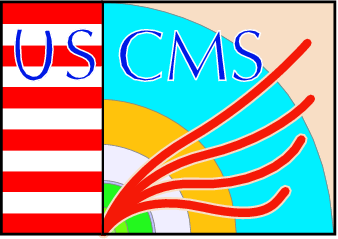
\includegraphics[height=0.6cm]{../../Graphics/USCMS_logo.png}\hspace{.1cm}
\includegraphics[height=0.75cm]{../../Graphics/UW_logo.png}}

\begin{document}

\begin{frame}
    \titlepage
\end{frame}

\section{Overview}
\begin{frame}
    \tableofcontents
\end{frame}

\section{What's the LHC?}
\subsection{In Pictures}
\begin{frame}
\begin{center}
\includegraphics<1>[height=7cm]{Graphics/lhc-aerial.jpg}
\includegraphics<2>[height=7cm]{Graphics/proton.png}
\includegraphics<3>[height=7cm]{Graphics/blackhole.jpg}
\includegraphics<4>[height=7cm]{Graphics/higgs-event.jpg}

\textbf<1->{Large} \textbf<2->{Hadron} \textbf<3->{Collider}

\end{center}
\end{frame}

\subsection{Timeline}
\begin{frame}
How to get a Nobel Prize:
\begin{itemize}
    \item<1-> Design a big collider thingy (\ca{}5 years)
    \item<2-> Get your collider on a bunch of national budgets (\ca{}1 year)
    \item<3-> Build it with a couple thousand of your closest friends (\ca{}15 years)
    \item<4-> Start it up
    \item<5-> Fix the broken transformers and magents and start it up again (\ca{}8 months)
    \item<6-> \ldots{} (??? years)
    \item<7-> Nobel!
\end{itemize}

\end{frame}

\subsection{Collider}
\subsection{Detectors}
\subsection{Grid}

\section{What's Wisconsin's role?}
\subsection{Trigger}
\subsection{Tier2 data center}

\section{Linux and the LHC}
\subsection{WAN transfers}
\subsection{Computation}
\subsection{Storage}
\subsection{Monitoring and Infrastructure}

\end{document}
